
\section{Running Example}

In order to illustrate the issues with existing notebooks and describe the extensions in \projname\, we will use the following example of a potential analysis:

\begin{example}
Consider a data analyst, working for a news portal website. The analyst wishes to create a notebook that extracts and presents information about the demographics of the website's reader-base during particular hours. More specifically, the analyst wants to construct a chart showing the number of readers that visit the website during the day; then based on this information, she would like to extract the age groups of the visitors, during various hours of that day and present the results to the portal editor. Figure \ref{figure:first-running-example:first-line-chart} shows the graph that displays the number of visitors per hour in a line chart and Figure \ref{figure:first-running-example:first-bar-chart} displays the age groups of the visitors in a bar chart. By doing this, the analyst can convince the portal editor to publish more articles and advertisements that target particular age groups during hours in which they visit the portal the most, thus maximizing the portal's revenue and reader's satisfaction.
\end{example}

\begin{figure}[ht]
  \centering
  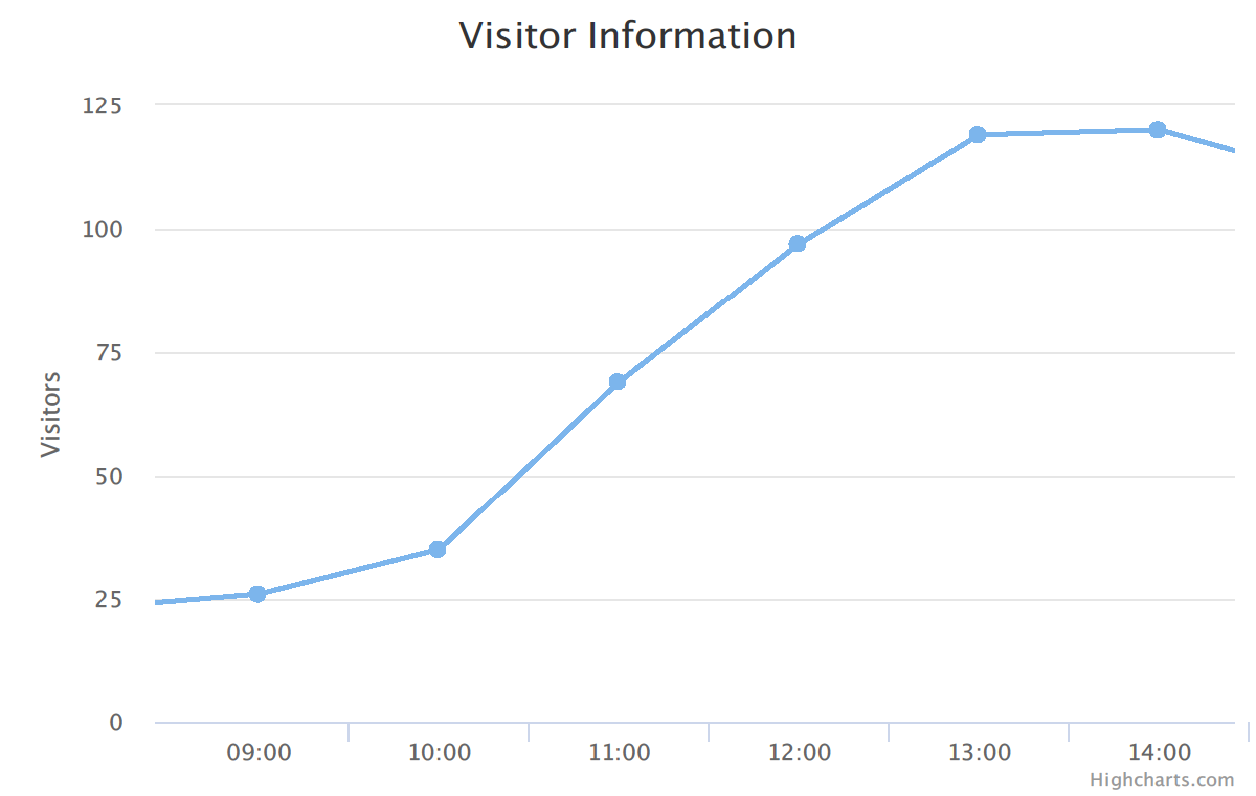
\includegraphics[width=0.8\columnwidth]{figures/first-line.png}
  \caption{Line chart showing visitors per hour}
\label{figure:first-running-example:first-line-chart}
  %\vspace*{\floatsep}% http://tex.stackexchange.com/q/26521/5764
   \vspace*{0.1cm}
  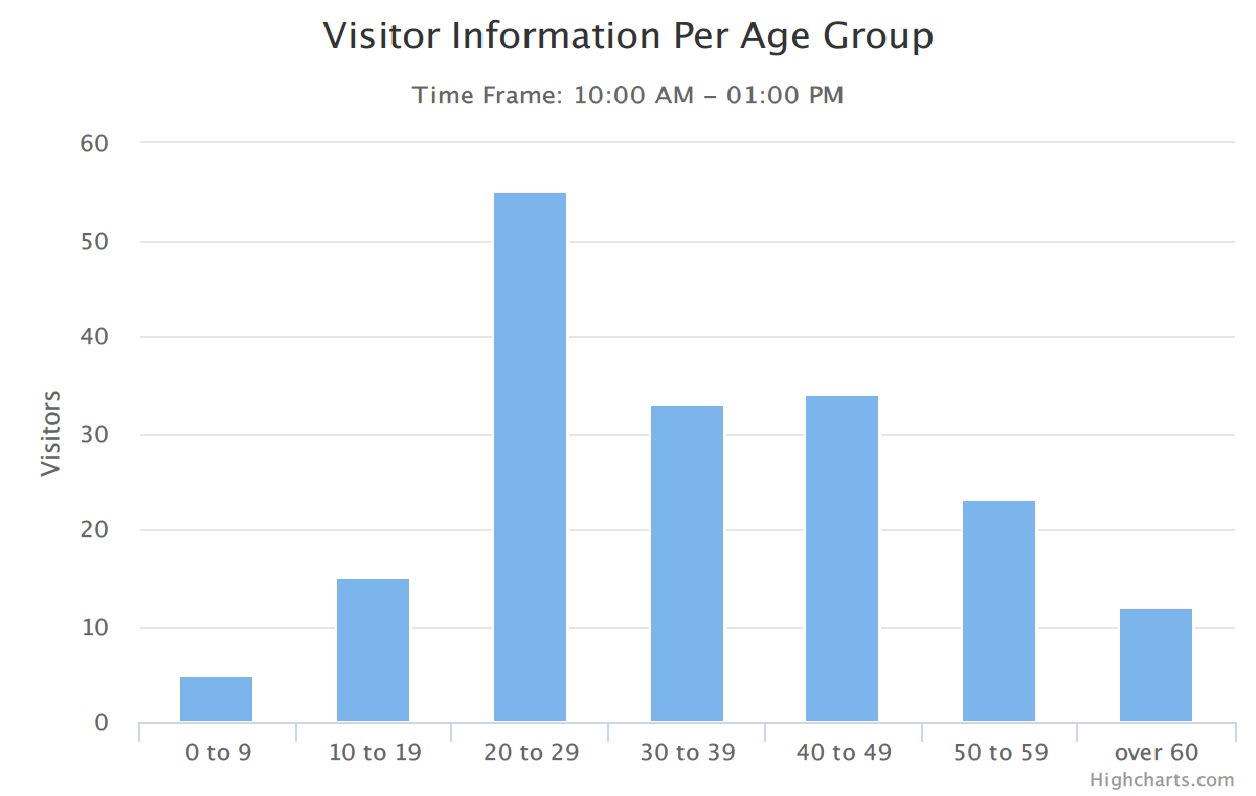
\includegraphics[width=0.8\columnwidth]{figures/first-bar.png}
  \caption{Bar chart showing age groups of visitors}
  \label{figure:first-running-example:first-bar-chart}
\end{figure}



For this analysis, we assume that the news portal maintains information about its reader-base in a Postgres database system. Table \ref{tab:schema} shows a potential database schema, that could be used for storing visitor information. The database contains two tables, namely ``Page Views" and ``Visitors"; table ``Visitors" contains information about each reader, such as the reader id, name, lastname, username and age. The table ``Page Views" maintains a tuple for each visit, and it consists of a visit id, the visitor id (foreign key referencing the visitor), the url of the visited page and the hour and date in which the user visited the website. The reader information could have been retrieved, with their permission, from various social media services (such as Facebook, Google etc). In order to construct this notebook, the data analyst must (a) retrieve  website access information from the database, by joining the two tables on the visitor id (b) generate a plot that shows the number of users that visit the website during the day, (c) issue a query that counts the number of visitors per age group, for each potential set of selected hours, and (d) create a bar chart that shows the number of visitors per age group. 


\section{Traditional Notebooks}



We will now describe how a data scientist would perform this analysis with a traditional interactive notebook that uses Python. While we do so, we will describe the issues that arise.

\noindent {\bf Setting up and interacting  with third-party utility libraries - Security concerns.} Before even starting working on any of the afore-mentioned tasks the data analyst must make sure that all third-party python packages that will be used for retrieving and visualizing data, are installed. This step will either introduce a dependency between the analyst and some system administrator, or the analyst will need the appropriate access rights in order to perform the installation, typically, using a command line. The latter can be a security concern (especially, if the server on which the notebook operates, also hosts other applications) and can also lead to corrupted systems if not performed correctly. The complexity of this step increases as the number of utility libraries, our analyst wants to use, increases. \eat{More specifically, for cases when an analyst needs to access data stored in a MongoDB and a MySQL database, two drivers will need to be installed.}

\begin{table}
\begin{center}

\begin{tabular}{|c|c|c|c|c|}
\hline 
\multicolumn{5}{|c|}{Page Views} \\ 
\hline 
id & vid & url & time & date \\ 
\hline 
\end{tabular} 

\hfill

\begin{tabular}{|c|c|c|c|c|}
\hline 
\multicolumn{5}{|c|}{Visitors} \\ 
\hline 
vid & name & lastname & username & age \\ 
\hline 
\end{tabular} 

\end{center}
\caption{Schema description of the two tables in our database.}
\label{tab:schema}
\end{table}


Once the system is configured, the analyst needs to read lengthy documentation pages in order to properly issue queries to the employed database system, using the API of the respective library. This step typically requires the use of imperative code that interacts with the library. During this step, the analyst has to also specify the credentials that will be used for accessing the database system. In most such libraries, the credentials have to be inlined into the method call that establishes the connection with that system. While this would not be a security concern in a python application (since the code that includes the credentials would have been compiled into a binary file, thus hiding the credentials), in a python notebook, the credentials would lie in plain sight for anyone, who has access to the notebook, to see.

\noindent {\bf Data model conversions.}
After, establishing the connection with the database system, and issuing the queries, the analyst, is able to consume the results by using the internal, to the library, datamodel. After doing so, the analyst has to again read documentation pages in order to infer the data model dictated by the visualization library she selected, and manually perform the appropriate conversions in order to construct the first visualization, by invoking the appropriate renderer function. Note that data model conversions have to take place every time the analyst wishes to integrate a third-party library in her analysis, so the amount of plumbing code required, can quickly skyrocket.


\noindent {\bf Limited interactive exploratory capabilities.}
The next step, is for the analyst to issue a query that counts the visitors per age group for a set of selected hours and construct a bar chart showing the result. Note, however, that there's no straightforward way for selecting a meaningful time frame. The analyst will have to go through a process of trial and error, by issuing an arbitrary number of such queries and plotting the results, until she finds a set that produces valuable insight. Furthermore, even if the analyst goes through this process for the data corresponding to a particular day, the time frame selection she made, might not produce any valuable insight for the dataset corresponding to another day. Additionally, the reader cannot test further hypotheses she might have.

\subsubsection*{Discussion about reactive charts.} The use of co-dependent reactive charts would have been proven useful in this scenario. If the analyst was able to use a chart that allows the reader to select a particular range of hours by using the first plot, she could use that input in order to retrieve and plot only the user demographics for this particular range. Figure \ref{fig:reactive-data-processing} graphically depicts this process. The first figure shows the reader of the notebook, selecting a particular time frame; this causes the line chart to zoom in, thus showing only the selected time frame. After the update of the first chart, the subsequent bar chart is also updated thus only showing the age groups of the visitors in the selected time frame. This feature would add useful exploratory capabilities, to the notebook, which would be of great value to notebook readers. It would enable them to further analyze the dataset used by the notebook by simply interacting with the provided visualizations. 

It is important to note that this feature cannot be implemented currently in interactive notebooks. Instead, the analyst would have to implement a full blown application in order to enable non-technical users interact with visualizations in this way. This requires more time and effort as well as technical expertise with web frameworks that data analysts, might lack. This reactive behavior requires the implementation of actions that have to be invoked when particular mouse events take place on the pixels of the browser that correspond to the visualization. Additionally, such events have to take place in a specific order (mousedown-mousemove-mouseup) for the action to be invoked. The developer of such applications must install observers that listen for such events and then provide the application logic that asynchronously accesses the back-end database to retrieve new data based on the user's selection and then cause the appropriate mutations to the respective visualizations that depend on that data. 
\begin{figure}[]
\centering
	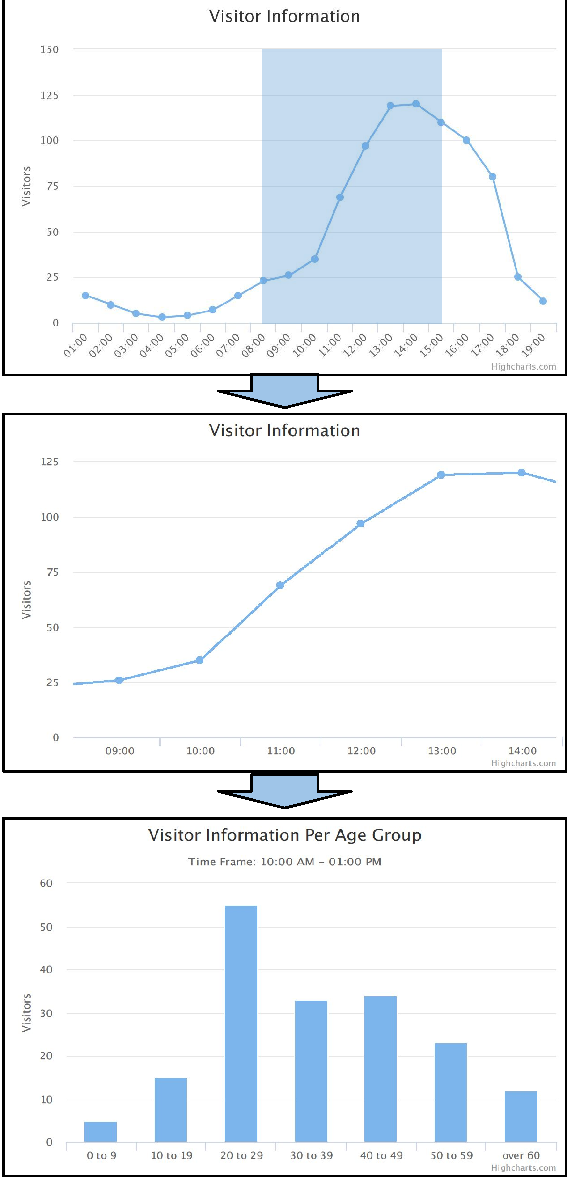
\includegraphics[width=0.7\columnwidth]{figures/reactive-processing.pdf}
	\caption{Demonstration of reactive charts. The reader's selection automatically updates both charts.}
	\label{fig:reactive-data-processing}
\end{figure}

 

\section{\projname\ Notebooks}

\projname\ notebooks provide constructs that simplify the process described in the last section. Firstly, \projname\ notebooks support two types of modules that simplify data access and visualizations, namely: \textbf{source wrappers} and \textbf{visual units}. Since these modules come preinstalled with \projname\ notebooks, analysts do not need to install any third-party packages in order to retrieve or visualize data.

% Template and template instance figures
\begin{figure*}
\centering
%
%
\begin{minipage}[c]{6cm}
%
\begin{minipage}[c]{6cm}
\begin{code}
\textbf{<\% let} readings = 
   SELECT count(time) as visits, time
   FROM (SELECT * FROM page_views pv 
  	     join visitors v 
         on pv.v_id = v.vid) AS joined_table
   GROUP BY time 
   ORDER BY time ASC \textbf{\%>}
\end{code}
\vspace*{-0.4cm}
\subcaption{Data retrieval}
\label{figure:first-running-example:data-retrieval}
\vspace*{0.3cm}
\end{minipage}



\begin{minipage}[c]{6cm}
\begin{code}
readings = [
   \{visits: 15, time: '08:00'\}, 
   \{visits: 10, time: '09:00'\},
   \{visits: 25, time: '10:00'\},  ...]
\end{code}
\vspace*{-0.4cm}
\subcaption{Query Result}
\label{figure:running-example:query-result}
\vspace*{0.3cm}
\end{minipage}


\begin{minipage}[c]{6cm}
\begin{code}
   sources : [ \{ 
     driver   : "postgres", 
     host     : "edu.db.domain", 
     expose   : [ \{
      schema : 'website_info', 
      tables: [visits, page_views] \} ]
     port     : 5432, 
     username : "dbadmin" 
     password : 'myP@ss'
   \}] 
\end{code}
\vspace*{-0.4cm}
\subcaption{DB Access Configuration file}
\vspace*{0.3cm}
\label{figure:source-config-file}
\end{minipage}
%
\vspace*{0.6cm}
\end{minipage}
\hspace{2cm}
\begin{minipage}[c]{6cm}
\begin{minipage}[c]{7.5cm}
\begin{code}
  \directive{unit}{highcharts} \{
    title: 'Visitor information' ,
    type: 'line',
    xAxis : \{ 
      labels : ['08:00','09:00'...],
      min : '08:00'
      max : '22:00'
    \}
    series: [\{ data: [ \{y:15\}, \{y:10\}...] \}]
  \} \directive{end unit}{}
\end{code}
\vspace*{-0.4cm}
\subcaption{Unit with evaluated unit state}
\vspace*{0.3cm}
\label{figure:running-example:unit-body}
\end{minipage}
\begin{minipage}[c]{7.5cm}
\begin{code}
  \directive{unit}{highcharts} \{
    title: 'Visitor information',
    type: 'line',
    xAxis : \{ 
      labels : [
        \directive{for}{reading \textbf{in} readings} 
          \directive{print}{reading.time} 
        \directive{end for}{}],
      min : \directive{bind}{min_time},
      max : \directive{bind}{max_time}
    \}
    series: [\{
      data: [ \directive{for}{reading \textbf{in} readings}
          \{
            y  : \directive{print}{reading.count}
          \}
        \directive{end for}{} ]
    \}]
  \} \directive{end unit}{}
\end{code}
\vspace*{-0.3cm}
\subcaption{Template \texttt{temp\_view}}
\vspace*{0cm}
\label{figure:first-running-example:main-template}
\end{minipage}
\end{minipage}
\vspace*{-0.3cm}
\caption{Template, template instance, and UAS configuration file for the running example}
\vspace*{-0.3cm}
\end{figure*}


\subsubsection*{Source wrappers}

Source wrappers allow the use of source specific languages for querying database systems (for instance SQL can be used to query MySQL and PostgreSQL databases, N1QL for Couchcase etc.). When using a \projname\ notebook, data analysts can directly provide a query on the notebook interface. This query is automatically used by the appropriate source wrapper, that evaluates it, propagates it to the respective data base system and returns the result in JSON format. This result is automatically assigned to a variable which can later be used in subsequent parts of the notebook (as will be described later in this section). Figure \ref{figure:first-running-example:data-retrieval} contains the first query of our analysis. It joins the two tables: $visitors$ and $page\_views$ on the id of the visitor, then groups the result on the $time$ attribute and runs a $count$ aggregate to count the visitors per unit of time. Lastly, it sorts the resulting dataset by time in ascending order and assigns the result into a \projname\ variable. Figure \ref{figure:running-example:query-result} shows the result of this query. Notice that the result has been converted into a JSON array by the respective source wrapper. 

In order for source wrappers to connect to the respective database systems, the data analyst must also provide a configuration file, describing the information required for establishing a connection with each source. Such configuration files are added from the interface of the notebook. Once added, these files are hidden from the UI and encrypted thus diminishing any security concerns. Figure \ref{figure:source-config-file} shows a sample configuration file that is used for accessing a postgres database that contains the data that will by used in our analysis. The configuration file must include the type of the database system, the host name, port and the credentials that will be used for obtaining a connection. Additionally, it must contain the database tables that will be accessible by queries. Only the tables that are explicitly defined in the configuration file will be accessible in the notebook. Once imported, this file is evaluated by the \projname\ engine and the schema of the accessible tables is displayed on the notebook, thus allowing the notebook user to get a glimpse of that information when generating the queries. 


\subsubsection*{Visual Units}
\eat{Once data analysts have obtained the data with the use of source wrappers, they can feed them into visual units in order to generate the respective visualizations. }Visual units are constructs capable of generating fully reactive visualizations, that take advantage of the advanced interactive capabilities of modern browsers. In the eyes of an analyst a visual unit is simply a black box that takes as input a JSON value that describes the state of the visualization. This JSON value is called \emph{unit instance}. The visual unit internally uses the unit instance to invoke the appropriate renderer calls that will generate the expected visualization. A particular instantiation of the unit  can be described as $\gl{<\% unit } U \gl{ \%> } v \gl{ <\% end unit \%>}$, where $U$ the type of the visual unit and $v$ the JSON value corresponding to the unit instance. Figure \ref{figure:running-example:unit-body} shows the unit instance of type \texttt{highcharts}, that is used to generate the visualization shown in Figure \ref{figure:first-running-example:first-line-chart}. The unit instance describes all the information that will be displayed in the visualization (such as the type and title of the chart, the labels on the x axis and so on). Each visual unit, comes with a unit instance schema that describes the format of the unit instance. As the reader interacts with visualizations, she can trigger mutations in the unit instance. For example, if the reader selects a particular area of the chart generated by the unit instance shown in Figure \ref{figure:running-example:unit-body}, the min and max attributes (in lines 6-7) will be updated accordingly.


\begin{figure*}
\centering
%
%
\begin{minipage}[c]{7.5cm}
%
\begin{minipage}[c]{7.5cm}
\begin{code}
\textbf{<\% let} age_groups = 
   SELECT agegroup, count(*) AS total 
   FROM (SELECT CASE
    WHEN age BETWEEN 0 AND 9 THEN '0 to 9'
    WHEN age BETWEEN 10 and 19 THEN '10 to 19'
     ...
    FROM (SELECT * FROM page_views pv join visitors v 
          on pv.v_id = v.vid where time BETWEEN 
          \directive{print}{min_time} and 
          \directive{print}{max_time}) joined_data) jd
   GROUP BY agegroup  
   ORDER BY agegroup ASC \textbf{\%>}
\end{code}
\vspace*{-0.4cm}
\subcaption{Data retrieval}
\label{figure:running-example:age-group-data-retrieval}
\vspace*{0cm}
\end{minipage}

\begin{minipage}[c]{7.5cm}
\begin{code}
age_groups = [
   \{age_group: '0 to 9', total: 12\}, 
   \{age_group: '10 to 19', total: 67\},
   \{age_group: '20 to 29', total: 84\},  ...]
\end{code}
\vspace*{-0.4cm}
\subcaption{Query Result}
\label{figure:running-example:age-group-query-result}
\vspace*{-0.2cm}
\end{minipage}
%
\end{minipage}
\hspace{1cm}
\begin{minipage}[c]{6cm}

\begin{minipage}[c]{8.5cm}
\begin{code}
  \directive{unit}{highcharts}
  \{
    title: 'Visitor information',
    type: 'bar',
    xAxis : \{ 
      labels : [
        \directive{for}{v \textbf{in} age_groups} 
          \directive{print}{v.age_group} 
        \directive{end for}{}]
    \}
    series: [\{
      data: [ \directive{for}{v \textbf{in} age_groups}
          \{
            y  : \directive{print}{v.total}
          \}
        \directive{end for}{} ]
    \}]
  \}
  \directive{end unit}{}
\end{code}
\vspace*{-0.4cm}
\subcaption{Template \texttt{temp\_view}}
\vspace*{0cm}
\label{figure:running-example:age-group-template}
\end{minipage}
\end{minipage}
\vspace*{-0.05cm}
\caption{Template, template instance, and UAS configuration file for the running example}
\vspace*{-0.3cm}
\end{figure*}

\subsubsection*{Templates}
\label{section:template}


\eat{
\begin{figure}[t]
\centering
\scriptsize
\begin{tabular}{B}
\hline
 1  & \gn{template}             & \gp   & \gl{<\% template} \gn{template\_name} (\gn{param\_list}) \gl{\%>}                    \\
    &                           &       & ~~ \gn{let}*                                    \\
    &                           &       & ~~ \gn{unit}
\\
    &                           &       & \gl{<\% end template \%>}                                         \\
 2  & \gn{param\_list}			& \gp   & ( \gn{var\_name} (, \gn{var\_name})* )? 
\\ \hline
 3  & \gn{unit}         & \gp   & \gl{<\% unit} \gn{unit\_class} \gl{\%>}               \\
    &                           &       & ~~ \gn{value}                                         \\
    &                           &       & \gl{<\% end unit \%>}                                 \\
 4  & \gn{value}                & \gp   & \gn{jsonpp\_value} %\text{(see Figure~\ref{figure:bnf-value})} 
\\
 5  &                           & \gd   & \gn{unit}                                     
\\
 6  &                           & \gd   & \gn{print}                                                        \\
 7  &                           & \gd   & \gl{[} \gn{for} \gl{]}                                                                                \\
 8  &                           & \gd   & \gl{<} \gn{for} \gl{>}                                                                                \\
 9  &                           & \gd   & \gn{if}                                                                                 \\
  
 10  &                           & \gd   & \gn{bind}                                                         \\
11  &                           & \gd   & \gl{\{} \gn{event}*                                               \\
    &                           &       & ~~ (\gl{\textquotedbl}\gn{string}\gl{\textquotedbl} 
                                             \gl{:} \gn{value}                                              \\
    &                           &       & ~~ (\gl{,} \gl{\textquotedbl}\gn{string}\gl{\textquotedbl} 
                                             \gl{:} \gn{value})* )? \gl{\}}                                           \\ \hline
12  & \gn{let}                 & \gp   & \gl{<\% let} \gn{var\_name} \gl{=} \gn{expr} \gl{\%>}            
\\
13  & \gn{print}                & \gp   & \gl{<\% print} \gn{expr} \gl{\%>}                                 \\
14  & \gn{for}                  & \gp   & \gl{<\% for} \gn{var\_name} \gl{in} \gn{expr} \gl{\%>}           
\\
    &                           &       & ~~ \gn{let}*                                    \\
    &                           &       & ~~ \gn{value}
\\
    &                           &       & \gl{<\% end for \%>}                                              \\
    
14  & \gn{if}                  & \gp   & \gl{<\% if}  \gn{expr} \gl{\%>}           
\\
    &                           &       & ~~ \gn{value}
\\
 &                           &       & ~~ (\gl{<\% elif}  \gn{expr} \gl{\%>} 
 
\\
 &                           &       & ~~ \gn{value})*    
 \\
 &                           &       & ~~ (\gl{<\% else}  \gl{\%>} 
 
\\
 &                           &       & ~~ \gn{value})?    
\\
    &                           &       & \gl{<\% end if \%>}                                              \\
15  & \gn{bind}                 & \gp   & \gl{<\% bind} \gn{var\_name} = \gn{expr} \gl{\%>}                             \\
16  & \gn{event}                & \gp   & \gl{<\% event} \gn{event\_name} \gn{action\_name} \gl{\%>}        \\
17  & \gn{expr}                 & \gp   & \gn{js\_expression}                                               \\
18  &                           & \gd   & \gn{source\_expression}                                                   \\
19  &                           & \gd   & \gn{json\_path}                                                   \\
\hline
\end{tabular}
\caption{BNF Grammar for Templates}
\label{figure:bnf-template}
\end{figure}
}


Despite the fact that both source wrappers and visual units use the JSON data model, data scientists often need to perform additional computation or simply transformations on JSON data. In order to facilitate this process, without requiring the use of imperative logic, \projname\ provides a declarative template language that operates on JSON data. 



Formally, \emph{Templates} are declarative specifications that can be used to generate JSON variables, parameterized queries or unit instances. The template language supports a set of \emph{template directives}, all of which operate on the JSON data model. Due to lack of space we do not include a formal definition of the grammar, instead we simply describe each of them in detail and provide a concrete example that illustrates their use. 




\noindent {\bf Defining variables.} A template may define variables that are added to the notebook's environment so that they can be used in subsequent statements. The $\gl{<\% let } x \gl{ = } E \gl{ \%>}$ directive defines variable $x$ and assigns to it the result of the expression $E$. $E$ can denote four types of expressions: (a) path navigation on JSON data, (b) invocation of a python function that performs computation by using as input and output JSON values, (c) another subexpression containing directives that report data (defined in the next subsection) or (d) a source-specific language with nested reporting directives (such as a SQL query). For instance, the template shown in Figure \ref{figure:first-running-example:data-retrieval} employs a \gl{let} directive to create a variable \texttt{readings} containing the visitor information that will be displayed in the chart (retrieved from a relational DBMS through an SQL query).

\noindent {\bf Reporting data.} Value assignments and iterations over collections are specified by using the \gl{print} and \gl{for} directives. The $\gl{<\% print } E \gl{ \%>}$ directive evaluates the expression $E$ and returns the result, while the $\gl{<\% for } x \gl{ in } E \gl{ \%> } B \gl{ <\% end for \%>}$ directive specifies that variable $x$ iterates over the result of $E$ and, in each iteration, it instanciates the body $B$ of the \gl{for} loop. Specifically, in Figure \ref{figure:first-running-example:main-template}, in lines 6-8 and 13-17 a \gl{for} directive is used to iterate over the readings retrieved from the database and for each reading, it generates a new JSON value, with the use of the \gl{print} directive. Particularly, in line 7 the template generates a string (the time label), which is added to the labels array (which contains the labels that will appear on the x axis of the chart). In lines 14-16 it generates a JSON object of the form \{y: ...\} and adds it to the data array. The data array in highcharts contains the points that will appear in the chart.

\eat{
\noindent {\bf Collecting data.} In addition to specifying how to compute a template instance, the template's \gl{bind} directive allows the analyst to specify user input collection. Specifically, the $\gl{<\% bind x} \gl{ \%>}$ directive describes a two-way bind that will be created between the part of the unit instance appearing on its left side and to variable $x$. For instance, in Figure \ref{figure:first-running-example:main-template} in lines 10-11 we create a two-way binding between the min and max boundaries of the chart and the min and max values of the time labels that have been retrieved (namely min\_time and max\_time). While the user interacts with chart he can select a particular region in the chart which in turn updates the values $min\_time$ and $max\_time$. This event invokes an internal propagation algorithm (which will be described in the next section) which triggers the revaluation of the \projname\ statements that use the values $min\_time$ and $max\_time$ in other parts of the notebook.
}





\noindent {\bf Collecting data.} The template's \gl{bind} directive allows the analyst to specify user input collection. Specifically, the $\gl{<\% bind x} \gl{ \%>}$ directive describes a two-way binding between the part of the unit instance appearing on the left side of the directive and the variable $x$. Once the reader interacts with the generated visualization and causes mutations to the underlying unit instance, these mutations will be propagated to the respective bound variables. For instance, in Figure \ref{figure:first-running-example:main-template} in lines 9-10 we create a two-way binding between the min and max boundaries of the chart and the min and max values of the time labels that have been received from the database (namely min\_time and max\_time). As the reader interacts with the generated chart she can select a particular time frame by dragging and dropping the mouse over a region. This action updates the min and max attributes of the unit instance which in turn updates the values $min\_time$ and $max\_time$. 

\eat{
This event invokes an internal propagation algorithm (which will be described in the next section)  triggers the revaluation of the \projname\ statements that use the values $min\_time$ and $max\_time$ in other parts of the notebook.

For instance, the template shown in Figure \ref{figure:first-running-example:main-template} contains two variables, namely $min\_time$ and $max\_time$, which are bound to the $min$ and $max$ unit instance attributes respectively. These variables are later used in the parameterized query shown in Figure \ref{figure:running-example:age-group-data-retrieval} which retrieves information about the users that visited the website in the time-frame specified by $min\_time$ and $max\_time$, groups the result in age groups and sums up the visits made by each age group. Figure \ref{figure:running-example:age-group-query-result}, contains the result of that query. This result is assigned to variable $age\_groups$ which is then used to produce the bar chart appearing in Figure \costas{add Figure} (the template shown in Figure \ref{figure:running-example:age-group-template} shows the template that created that chart)
}
\subsubsection*{Internal Data Model \&  Propagation Algorithm}
\label{section:change-propagation-datamodel}




Once a set of bound variables is mutated by a visual unit as a result of reader interaction, \projname\ is responsible for reflecting these changes to all other parts of the notebook that depend on those variables. For instance, in Figure \ref{figure:running-example:age-group-data-retrieval} we show a parameterized query that collects all users that visited the website in the time-frame specified by $min\_time$ and $max\_time$, then categorizes them into age groups and lastly counts the users that correspond to each age group. The result of this query is assigned to the variable $age\_groups$ (Figure \ref{figure:running-example:age-group-query-result} shows the contents of this variable). The variable $age\_groups$ is then used in the template shown in Figure \ref{figure:running-example:age-group-template} (lines 7-9 and 12-16) to produce the bar chart appearing in Figure \ref{figure:first-running-example:first-bar-chart}. In this scenario, if the reader's interaction with the chart shown in Figure \ref{figure:first-running-example:first-line-chart}, caused the mutation of variables $min\_time$ and $max\_time$, then \projname\ must trigger a chain reaction that causes the reevaluation of both the query and the following visualization in order to reflect the changes. We will now describe this process.



% which categorizes the users that visited the website in the time-frame specified by $min\_time$ and $max\_time$ by age groups and then sums up the visits made by each age group. Figure \ref{figure:running-example:age-group-query-result}, contains the result of that query. This result is then assigned to variable $age\_groups$ which is then used to produce the bar chart appearing in Figure \ref{figure:first-running-example:first-bar-chart} (the template shown in Figure \ref{figure:running-example:age-group-template} shows the template that created that chart)


\eat{
the template shown in Figure \ref{figure:first-running-example:main-template} contains two variables, namely $min\_time$ and $max\_time$, which are bound to the $min$ and $max$ unit instance attributes respectively. These variables are later used in the parameterized query shown in Figure \ref{figure:running-example:age-group-data-retrieval} which retrieves information about the users that visited the website in the time-frame specified by $min\_time$ and $max\_time$, groups the result in age groups and sums up the visits made by each age group. Figure \ref{figure:running-example:age-group-query-result}, contains the result of that query. This result is assigned to variable $age\_groups$ which is then used to produce the bar chart appearing in Figure \costas{add Figure} (the template shown in Figure \ref{figure:running-example:age-group-template} shows the template that created that chart)
}



\eat{Since, as explained above, \projname\ variables are represented using JSON, changes to either of them are represented as diffs.}
\noindent{\bf Internal Data Model - Diffs} \\ Once a variable is mutated by a unit, a diff is also generated to describe this mutation. A \emph{diff} is the internal data model that is shared between visual units and the change propagation algorithm, this data model is hidden from data analysts and notebook readers. A diff that targets a JSON value is of the form $\diff{}{}{\pp{p}}$, where $\pp{p}$ is the path to the element that is being modified. 

\eat{The first token, $f$ of that path $\pp{p}$ denotes the variable that is being mutated; if the diff contains information about mutations on particular attributes or elements of the variable, then $f$ is followed by more tokens. Specifically, in order to describe a mutation on an individual attribute $k$ of a JSON value identified by path $p$ we use the notation $p.k$ and in order to describe the $i$-th element of the array targeted by a path $p$ we use the notation $p[k]$.}

\noindent{\bf Change Propagation Algorithm.}\\
Once a diff is generated for each mutated variable \projname\ invokes the change propagation algorithm. Algorithm \ref{algo:change-propagation-algorithm2} summarizes this change propagation algorithm. The algorithm takes as input a set of diffs, and invokes the reevaluation of all statements that depend on the targeted variables. Specifically, it iterates over each statement of each coding snippet that appears in the notebook (as shown in line 2) and performs the following checks:

\begin{itemize}
\item If the statement defines a new variable $x$ (line 3), then the algorithm visits every sub-expression of the \gl{let} directive and checks if it is targeted by any diff in D (line 4). If there is, the change propagation algorithm causes the reevaluation of the $\gl{let}$ statement (line 5), updates the notebook environment with the new value of x (line 6) and lastly constructs a new diff that targets x (line 7)

\item If the statement constructs a visualization using a visual unit of type U with body B (line 8), then the algorithm visits every sub-expression in body B and checks if it is targeted by any diff in D (line 9). If there is, the change propagation algorithm causes the reevaluation of the entire body B, thus generating the unit instance r and then reinvokes the unit U with new unit instance (line 10).



\end{itemize}

\eat{

\begin{figure*}
\centering
%
%
\begin{minipage}[c]{7.5cm}
%
\begin{minipage}[c]{7.5cm}
\begin{code}
\textbf{<\% let} age_groups = 
   SELECT agegroup, count(*) AS total 
   FROM (SELECT CASE
    WHEN age BETWEEN 0 AND 9 THEN '0 to 9'
    WHEN age BETWEEN 10 and 19 THEN '10 to 19'
     ...
    FROM (SELECT * FROM page_views pv join visitors v 
          on pv.v_id = v.vid where time BETWEEN 
          \directive{print}{min_time} and 
          \directive{print}{max_time}) joined_data) jd
   GROUP BY agegroup  
   ORDER BY agegroup ASC \textbf{\%>}
\end{code}
\vspace*{-0.4cm}
\subcaption{Data retrieval}
\label{figure:running-example:age-group-data-retrieval}
\vspace*{0cm}
\end{minipage}

\begin{minipage}[c]{7.5cm}
\begin{code}
age_groups = [
   \{age_group: '0 to 9', total: 12\}, 
   \{age_group: '10 to 19', total: 67\},
   \{age_group: '20 to 29', total: 84\},  ...]
\end{code}
\vspace*{-0.4cm}
\subcaption{Query Result}
\label{figure:running-example:age-group-query-result}
\vspace*{-0.2cm}
\end{minipage}
%
\end{minipage}
\hspace{1cm}
\begin{minipage}[c]{6cm}

\begin{minipage}[c]{8.5cm}
\begin{code}
  \directive{unit}{highcharts}
  \{
    title: 'Visitor information',
    xAxis : \{ 
      labels : [
        \directive{for}{v \textbf{in} age_groups} 
          \directive{print}{v.age_group} 
        \directive{end for}{}]
    \}
    series: [\{
      data: [ \directive{for}{v \textbf{in} age_groups}
          \{
            y  : \directive{print}{v.total}
          \}
        \directive{end for}{} ]
    \}]
  \}
  \directive{end unit}{}
\end{code}
\vspace*{-0.4cm}
\subcaption{Template \texttt{temp\_view}}
\vspace*{0cm}
\label{figure:running-example:age-group-template}
\end{minipage}
\end{minipage}
\vspace*{-0.05cm}
\caption{Template, template instance, and UAS configuration file for the running example}
\vspace*{-0.3cm}
\end{figure*}
}


\eat{
\begin{itemize}
\item First, if the statement defines a new variable $x$ by using a $\gl{let}$ directive, and the expression of $\gl{let}$ contains at least one reporting directive (either a $\gl{for}$ or a $\gl{print}$), then the algorithm checks whether there is a diff that targets any of the expressions of the reporting directives. If there is, the change propagation algorithm causes the reevaluation of the $\gl{let}$ statement, updates the notebook environment with the new value of x and constructs a new diff that targets x
\item 2 if the statement defines a new variable $x$ by using a $\gl{let}$ directive, and the expression of $\gl{let}$ contains at least one for $\gl{for}$ the body of which contains some , then the algorithm checks whether there is a diff that targets any of the expressions of the reporting directives. If there is, the change propagation algorithm causes the reevaluation of the $\gl{let}$ statement, updates the notebook environment with the new value of x and constructs a new diff that targets x
\item 3

\end{itemize}
}

\begin{algorithm}[t!]
    \SetKwProg{Function}{function}{}{}
    \SetKwFunction{changepropagation}{change-propagation}
    \SetKwFunction{IVMPath}{IVMPath}
    \SetKwFunction{prefixDiffs}{prefixDiffs}
    \SetKwFunction{navigate}{navigate}
    \SetKwFunction{keysWithin}{keysWithin}
    \SetKwFunction{instantiateTemplate}{instantiateTemplate}
    \SetKwFunction{instantiateVmPayload}{instantiateVmPayload}
    \SetKwFunction{instantiateForLoopVmPayload}{instantiateForLoopVmPayload}
    \Function{\changepropagation{Notebook $N$, Environment $env$, Set of Input Diffs $D$}}{
    	\For {\textbf{each} statement s in each coding snippet of N}{
	    		 \uIf  {s is $\gl{<\% let } x \gl{ = } E \gl{ \%>}$ } {
	    		  \uIf  {There is $\Delta^{}(t) \in D$ with $t$ that targets any subexpression of E} {
	    		    Reevaluate $E$ and assign result $r$ to $x$\;
	    		    Update $env$ with new value of $x$\;
	    		    Construct $\Delta^{}(x)$ and add it to D\;
	    		 }
    		 }
			 \uElseIf  {s is $\gl{<\%unit } U \gl{\%> } B \gl{ <\%end unit\%>}$ } {
			 	\uIf  {There is $\Delta^{}(t) \in D$ with $t$ that that targets any subexpression of B} {
			  		Reevaluate $B$ and invoke unit U with result $r$ \;
			 	}
             }    
        }
        
    }
\caption{Change Propagation Algorithm}
\label{algo:change-propagation-algorithm2}
\end{algorithm} 


%


\begin{algorithm}[t!]
    \SetKwProg{Function}{function}{}{}
    \SetKwFunction{changepropagation}{change-propagation}
    \SetKwFunction{IVMPath}{IVMPath}
    \SetKwFunction{prefixDiffs}{prefixDiffs}
    \SetKwFunction{navigate}{navigate}
    \SetKwFunction{keysWithin}{keysWithin}
    \SetKwFunction{instantiateTemplate}{instantiateTemplate}
    \SetKwFunction{instantiateVmPayload}{instantiateVmPayload}
    \SetKwFunction{instantiateForLoopVmPayload}{instantiateForLoopVmPayload}
    \Function{\changepropagation{Notebook $N$, Environment $env$, Set of Input Diffs $D$}}{
    	Set of output diffs $D_{out} \leftarrow$ empty bag\;
    	\For {\textbf{each} statement s in each block of N}{
	    		 \uIf  {s is $\gl{<\% let } x \gl{ = } E \gl{ \%>}$ and E contains directive: \gl{<\%}\text{\textbf{for} $v$ \textbf{in} $E''$}\gl{\%>} or directive: $\gl{<\% }\text{\textbf{print} $E'$}\gl{ \%>}$ } {
	    		  \uIf  {There is $\Delta^{}(t; p) \in D$ with $t$ that matches $E'$ or $E''$} {
	    		    Reevaluate $E$ and assign result $r$ to $x$\;
	    		    Update $env$ with new value of $x$\;
	    		    Construct $\Delta^{}(x; r)$ and add it to D\;
	    		 }
    		 }
			 \uElseIf  {s is $\gl{<\%unit } U \gl{\%> } B \gl{ <\%end unit\%>}$ and B contains directives \gl{<\%}\text{\textbf{for} $v$ \textbf{in} $E''$}\gl{\%>} or $\gl{<\%}\text{\textbf{print} $E'$}\gl{\%>}$ } {
			 	\uIf  {There is $\Delta^{}(t; p) \in D$ with $t$ that matches $E'$ or $E''$} {
			  		Reevaluate $E$ and invoke unit U with result $r$ \;
			 	}
             }    
        }
        
        
        
        \Return{$D_{out}$}\;
    }
\caption{MVVM-IVM}
\label{algo:templateIVM}
\end{algorithm}


\begin{algorithm}[t!]
    \SetKwProg{Function}{function}{}{}
    \SetKwFunction{MVVMIVM}{MVVMIVM}
    \SetKwFunction{IVMPath}{IVMPath}
    \SetKwFunction{prefixDiffs}{prefixDiffs}
    \SetKwFunction{navigate}{navigate}
    \SetKwFunction{keysWithin}{keysWithin}
    \SetKwFunction{instantiateTemplate}{instantiateTemplate}
    \SetKwFunction{instantiateVmPayload}{instantiateVmPayload}
    \SetKwFunction{instantiateForLoopVmPayload}{instantiateForLoopVmPayload}
    \Function{\MVVMIVM{Template $T$, Model $M$, Set of Input Diffs $D_{in}$}}{
    	Set of output diffs $D_{out} \leftarrow$ empty bag\;
    	\For {top-level directive $d \in T$}{
    		 d.path $\leftarrow$ path to d in template T \\
             \uIf  {d is $\gl{<\% }\text{print Path $\pp{e}$}\gl{ \%>}$} {
   				  $\Delta \leftarrow \IVMPath(\pp{e}, M, D_{in})$\;
				  $D_{out} = D_{out} \cup \{\prefixDiffs(d.path, \{\Delta\})\}$
             }
			 \uElseIf  {d is $\gl{<\% }\text{for Var y in  Path $\pp{e}$}\gl{ \%>} B \gl{<\% }\text{end for}\gl{\%>}$} {
   				  $\Delta^{type}_{}(\pp{t}; p) \leftarrow \IVMPath(\pp{e}, M, D_{in})$\;   			
   				\uIf{$\pp{t} = empty$} {	  
					\uIf {$type = update$} {
						Let $T'$ be the template rooted at $d$, where $\pp{e}$ is replaced by $p$\;
						$p' \leftarrow \instantiateTemplate(T', M)$\;
						$D_{out} = D_{out} \cup \{\Delta^{update}(d.path; p')\}$\;
					}
				}
				\uElseIf {$\pp{t} = [k] \text{ and } type = insert \text{ } array$} {
					$M' \leftarrow M \# \{y \leftarrow p\}$\;
					$p' \leftarrow \instantiateTemplate(B, M')$\;
					$D_{out} = D_{out} \cup \{\Delta^{insert}_{array}(d.path[k]; p')\}$\;					
				}
				\uElseIf {$\pp{t} = [k]\pp{s}$} {
					$D'_{in} \leftarrow D_{in} \cup \{\Delta^{type}(y\ \pp{s}; p)\}$\;
					$D_{nested}$ = \MVVMIVM($B$, $M$, $D'_{in}$)\;
					remove first path step of each diff in $D_{nested}$\;
					$D_{out} \leftarrow D_{out} \cup \prefixDiffs(d.path[k], D_{nested})$\;
				}
%				\uElseIf {$\Delta^{type}_{}(\pp{t}; p)$ is null }
%				{
					$D_{nested}$ = \MVVMIVM($B$, $M$, $D_{in}$)\;
					\uIf  {$D_{nested}$ not an empty bag} {
						$l \leftarrow$ length of array e targeted by Path $\pp{e}$\\
						\For { i in [0 ... l]}{
							$D_{out} \leftarrow D_{out} \cup \prefixDiffs(d.path[i], D_{nested})$\;
						}
%					}
					
				}
\BlankLine			
%				$D_{inner}$ = \MVVMIVM($B$, $M$, $D'_{in}$)\;
%				$D_{out} \leftarrow D_{out} \cup \prefixDiffs(d.path[*], D_{inner})$\;
             }    
        }
        
        
        
        \Return{$D_{out}$}\;
    }
\caption{MVVM-IVM}
\label{algo:templateIVM}
\end{algorithm}

\begin{algorithm}[t!]
    \SetKwProg{Function}{function}{}{}
    \SetKwFunction{IVMPath}{IVMPath}
    \SetKwFunction{prefixDiffs}{prefixDiffs}
    \SetKwFunction{navigate}{navigate}
    \SetKwFunction{keysWithin}{keysWithin}
    \SetKwFunction{instantiateVmPayload}{instantiateVmPayload}
    \SetKwFunction{instantiateForLoopVmPayload}{instantiateForLoopVmPayload}
    \Function{\IVMPath{Path Expression $\pp{e}$, Model $M$, Set of Input Diffs $D_{in}$}}{
%    	Set of output diffs $D_{out} \leftarrow$ empty bag\;
   			\For {\textbf{each} $\Delta^{type}(\pp{t}; p) \in D_{in}$} {
   				  		\uIf {$\pp{t}$ is $\pp{e}\pp{s}$} {
% 								$D_{out} \leftarrow D_{out} \cup \{\Delta^{type}(\pp{s}; p)\}$
								\Return{$\Delta^{type}(\pp{s}; p)$}   				  		
   				  		}
   				  		\uElseIf {$\pp{e}$ is $\pp{t}\pp{s}$} { 
   				  			\uIf{$type = update$} {
   				  				$p' \leftarrow \navigate(p, \pp{s})$
\;
%								$D_{out} \leftarrow D_{out} \cup \{\Delta^{type}(empty; p')\}$ 
								\Return{$\Delta^{update}(empty; p')$}
							}
							\uIf{$type = delete$} {
															\Return{$\Delta^{delete}(empty)$}
														}
							\uElse {
   				  				$p' \leftarrow \navigate(M, \pp{e})$
\;
%								$D_{out} \leftarrow D_{out} \cup \{\Delta^{update}(empty; p')\}$ 							
								\Return{$\Delta^{update}(empty; p')$} 												
							}
   				  		}
				  }
%        \Return{$D_{out}$}\;
        \Return{$null$}\;
    }
\caption{IVMPath}
\label{algo:IVMExpression}
\end{algorithm}




\eat{

This template language allows the invocation of functions. Regardless of whether these functions are defined by users or by third-party packages they must operate on the JSON data model, in order to be used in a template.

Source wrappers produce and visual units consume JSON. Since both these constructs use the JSON data model, no data model transformations are required by the analyst. This minimizes the amount of plumbing code required for generating an analysis. For cases when the data analyst wishes to perform some additional computation or perform data transformations, \projname\ also supports a declarative template language that operates on JSON data. This template language also allows the invocation of functions. Regardless of whether these functions are defined by users or by third-party packages they must operate on the JSON data model, in order to be used in a template.

\emph{Templates} are declarative specifications that can be used to generate \projname\ variables or unit instances. The template language supports a set of \emph{template directives}, all of which operate on the JSON datamodel. These directives are used to describe computation, define variables and set up data collection. Due to lack of space we do not include a figure containing a formal BNF grammar for the template language, instead we simply describe each of them in detail and provide a concrete example that illustrates their use. 




\noindent {\bf Defining variables.} A template may define variables that are added to the notebook's environment so that they can be used in subsequent computation. The $\gl{<\% let } x \gl{ = } E \gl{ \%>}$ directive defines variable $x$ and assigns to it the result of the expression $E$. $E$ can denote three types of expressions: path navigation on JSON data, invocation of a python function that performs computation by using as input and output JSON values or a source-specific language (such as a SQL query). For instance, the template shown in Figure \ref{figure:first-running-example:data-retrieval} employs a \gl{let} directive to create a variable \texttt{readings} containing the visitor information that will be displayed in the chart (retrieved from a relational DBMS through an SQL query).

\noindent {\bf Reporting data.} Value assignments and iterations over collections are specified by using the \gl{print} and \gl{for} directives. The $\gl{<\% print } E \gl{ \%>}$ directive evaluates the expression $E$ and returns the result, while the $\gl{<\% for } x \gl{ in } E \gl{ \%> } B \gl{ <\% end for \%>}$ directive specifies that variable $x$ iterates over the result of $E$ and, in each iteration, it instanciates the body $B$ of the \gl{for} loop. In Figure \ref{figure:first-running-example:main-template}, in lines 7-9 and 14-18 a \gl{for} directive is used to iterate over the readings retrieved from the database and for each reading, it generates a new JSON value, with the use of the \gl{print} directive. Particularly, in line 8 the template generates a string (the time label), which is added to the labels array (which contains the labels that will appear on the x axis of the chart). In lines 15-17 it generates a JSON object of the form \{y: ...\} and adds it to the data array. The data array in highcharts contains the points that will appear in the chart.

\noindent {\bf Collecting data.} In addition to specifying how to compute a template instance, the template's \gl{bind} directive allows the analyst to specify user input collection. Specifically, the $\gl{<\% bind x} \gl{ \%>}$ directive describes a two-way bind that will be created between the part of the unit instance appearing on its left side and to variable $x$. For instance, in Figure \ref{figure:first-running-example:main-template} in lines 10-11 we create a two-way binding between the min and max boundaries of the chart and the min and max values of the time labels that have been retrieved (namely min\_time and max\_time). While the user interacts with chart he can select a particular region in the chart which in turn updates the values $min\_time$ and $max\_time$. This event invokes an internal propagation algorithm (which will be described in the next section) which triggers the revaluation of the \projname\ statements that use the values $min\_time$ and $max\_time$ in other parts of the notebook.



that take as input JSON objects (in a predefined format) and generate visualizations on the notebook interface. By not requiring any low level imperative code for this task 

\label{section:visual Units}

\noindent To shield analysts from the low level coding required to generate visualizations, \projname\ abstracts out each visual component as a \projname\ \emph{visual unit} (or simply \emph{unit}). In the eyes of the analyst a visual unit is simply a black box that takes as input a JSON value that describes the visualization, namely, unit instance. The visual unit internally uses the unit instance to invoke the appropriate renderer calls that will generate the expected visualization. As such a particular instantiation of the unit  can be described as $\gl{<\% unit } U \gl{ \%> } v \gl{ <\% end unit \%>}$, where $U$ the type of the visual unit and $v$ the JSON value corresponding to the input of the unit. 


For instance, Figure \ref{figure:running-example:unit-body} shows a unit instance of type \texttt{highcharts}. The unit instance describes all the information that will be displayed in the visualization (such as the title of the chart, the labels on the x axis and so on). Each visual unit, comes with a unit instance schema that describes the format of the unit instance.




In order for source wrappers to connect to the respective database systems, the data analyst must provide a configuration file, describing the information required for establishing a connection with each source. Such configuration files are added by interacting directly with the notebook interface, therefore data analysts do not have to use a command line during setup. Once added, these files are hidden from the UI and encrypted thus diminishing any security concerns. Lastly, visual units are constructs that take as input JSON objects (in a predefined format) and generate visualizations on the notebook interface. 


Source wrappers produce and visual units consume JSON. Since both these constructs use the JSON data model, no data model transformations are required by the analyst. This minimizes the amount of plumbing code required for generating an analysis. For cases when the data analyst wishes to perform some additional computation or perform data transformations, \projname\ also supports a declarative template language that operates on JSON data. This template language also allows the invocation of functions. Regardless of whether these functions are defined by users or by third-party packages they must operate on the JSON data model, in order to be used in a template.

This language also allows data analysts tp describe reactive behavior. Specifically, by binding individual variables to certain parts of the visual unit, data analysts can collect information which can later be used in other parts of the notebook. By doing so, analysts can describe computation that depends on the reader's input. \projname's propagation algorithm, identifies statements that depend on such libraries and triggers their evaluation. This process leads to truly interactive notebooks, that react to the reader's input, thus enhancing the exploratory capabilities of traditional notebooks.
}
\eat{
Source wrappers require the instantiation of a configuration file, that describes the information required for establishing a connection with each source. Such configuration files are added by data analysts by interacting directly with the notebook interface. Once added, these files are hidden from the UI and encrypted thus diminishing any security concerns. Lastly, visual units are constructs that take as input JSON objects (in a predefined format) and generate visualizations on the notebook interface. 


Most importantly, source wrappers and visual units, both use the same data model JSON, so no data model transformations are required for retrieving and visualizing data. For cases when the data analyst wishes to perform some data transformations, \projname\ also supports a declarative template language.


Once a source wrapper receives a query, it propagates it to the respective database system, and then parses and returns the result in JSON format. Source wrappers require the instantiation of a configuration file, that describes the information required for establishing a connection with each source. Such configuration files are added by data analysts by interacting directly with the notebook interface. Once added, these files are hidden from the UI and encrypted thus diminishing any security concerns. Lastly, visual units are constructs that take as input JSON objects (in a predefined format) and generate visualizations on the notebook interface. 

Both source wrappers and visual units come pre-installed and can be used directly on the notebook without the installation of any additional packages. Additionally, since no method calls are required for accessing and visualizing data, the analyst does not have to read long documentation files before using them. Most importantly, source wrappers and visual units, both use the same data model JSON, so no data model transformations are required for retrieving and visualizing data. For cases when the data analyst wishes to perform some data transformations, \projname\ also supports a declarative template language.
}

\eat{
interactive chart implementation using imperative languages is not a trivial task and possibly beyond the coding skill set of an average data analyst. Such a task requires advanced coding skills and implementation of event listeners to capture the user's mouse input and asynchronously trigger execution of other functions that will update data and re-draw the second figure. As we show later in Section ??, the {\projname} framework is equipped with modules that can take care of the heavy work, while the analyst only needs to define ``bound'' (linked) variables.


Finally, 


plot a line chart of access count Vs timestamp, as well as a bar chart of access count Vs age groups, and (c) be able to select a time range from the line chart using mouse input and automatically filter and display data in the second plot to present age-group-based activity within the selected time frame. 


The data analyst can access historic data about the user base by directly querying the data base system. Table \ref{tab:schema} shows the database schema. The analyst's first task is to retrieve the data via database queries, join the two tables based on the visitor id (``vid'') key and group by (1) ``time'' and (2) ``age'' to prepare the data for the two plots.

Installing packages, transferring data and connecting with database systems requires technical knowledge that often exceeds the skill-set of a typical data scientist. Lastly, while such notebooks support the generation of visualizations with the use of the appropriate library



Throughout this paper, we present {\projname} via an example data analysis: We assume a scenario where a data analyst must (a) retrieve  website access information from a database, (b) plot a line chart of access count Vs timestamp, as well as a bar chart of access count Vs age groups, and (c) be able to select a time range from the line chart using mouse input and automatically filter and display data in the second plot to present age-group-based activity within the selected time frame. 

For our walkthrough example, we assume a Jupyter server where the analysts develop their notebooks and a different database server where data is stored. Table \ref{tab:schema} shows how our databases are organized. The analyst's first task is to retrieve the data via database queries, join the two tables based on the visitor id (``vid'') key and group by (1) ``time'' and (2) ``age'' to prepare the data for the two plots.

During the visualization stage, the analyst implements two ``linked'' plots in such a way that a range selection in the first plot \textit{automatically} (without re-executing code in the notebook) filters the data presented in the second plot. Figure \ref{fig:vision} illustrates the expected chart behavior. A time-frame selection in the first chart (10:00AM - 1:00PM) causes the second chart to only plot those accesses that occurred during the selected interval. 

It is important to note that this interactive chart implementation using imperative languages is not a trivial task and possibly beyond the coding skill set of an average data analyst. Such a task requires advanced coding skills and implementation of event listeners to capture the user's mouse input and asynchronously trigger execution of other functions that will update data and re-draw the second figure. As we show later in Section ??, the {\projname} framework is equipped with modules that can take care of the heavy work, while the analyst only needs to define ``bound'' (linked) variables.
}
